$if(has-frontmatter)$
\frontmatter
$endif$
%
% make plain pages empty
\makeatletter
  \let\ps@plain\ps@empty
\makeatother
\setlength{\headheight}{15pt}
\addtolength{\headwidth}{\marginparwidth}
\fancyhf{}
\fancyhead[LO]{\nouppercase{\rightmark}}
\fancyhead[RO]{\thepage}
\fancyhead[LE]{\thepage}
\fancyhead[RE]{\nouppercase{\leftmark}}
\renewcommand{\headrulewidth}{0pt}
\pagenumbering{alph}
\pagestyle{empty}
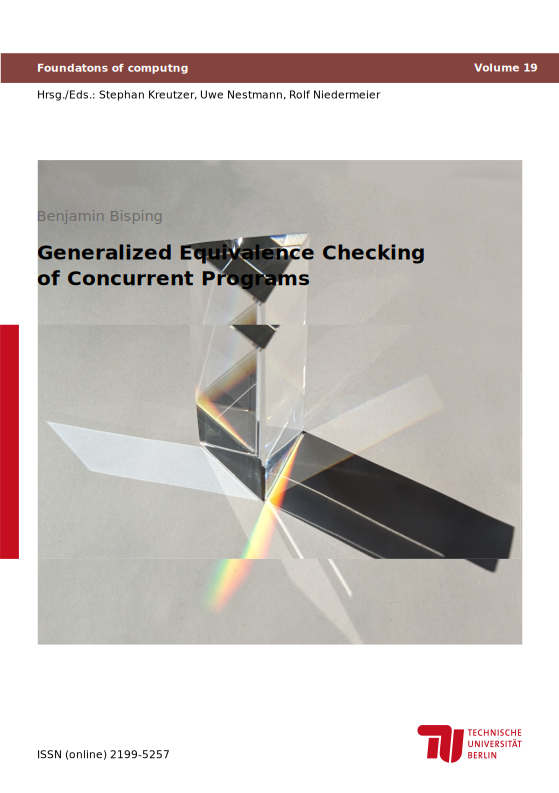
\includepdf{style-foc/cover.pdf}
\cleardoublepage
\pagestyle{fancy}
\pagenumbering{roman}
%\newgeometry{margin=4cm}
\begin{titlepage}
    \begin{center}
        \includegraphics[width=0.3\textwidth]{img/tu-berlin-logo-long-red.pdf}\\[5pt]
        \vspace{1cm}
        {\Large \(\triangle\)}\\[5pt]
        {\huge\bfseries Generalized Equivalence Checking \\ of Concurrent Programs\\}
        % --------s--------------------------------------------------------
        \vspace{.5cm}
        \vfill
        vorgelegt von\\[1em]
        {\Large\bfseries Benjamin Bisping \orcidlink{0000-0002-0637-0171}, M. Sc.}
        \\[5pt]
        \url{https://bbisping.de}\\[14pt]
        % -------------------------------------------
        \vfill
        an der Fakultät IV -- Elektrotechnik und Informatik\\
        der Technischen Universität Berlin\\
        zur Erlangung des akademischen Grades\\[1em]
        Doktor der Naturwissenschaften\\
        -- Dr. rer. nat. --\\[1em]

        genehmigte Dissertation
        \vspace{.5cm}
    \end{center}

    \noindent
    \begin{tabbing}
      \hspace*{7em}\=\hspace*{12em}\kill
      Promotionsausschuss:\\[1em]
      Vorsitzender: \> Prof. Dr. Stephan Kreutzer\\
      Gutachter: \> Prof. Dr.-Ing. Uwe Nestmann\\
      Gutachter: \> Prof. Dr. Rob J. van Glabbeek (University of Edinburgh, UK)\\
      Gutachter: \> Prof. Dr. ir. Jan Friso Groote (TU Eindhoven, Netherlands)\\
    \end{tabbing}

    \vspace{1em}

    \noindent
    Tag der wissenschaftlichen Aussprache: 28. Juli 2025\\

    \vfill

    \begin{center}
        Berlin 2025\\[1em]
    \end{center}

\end{titlepage}
\restoregeometry

\newpage
\thispagestyle{empty}
\noindent
\textbf{Foundations of computing \quad | \quad 19}

\vspace{0.5cm}

\noindent
The scientific series \emph{Foundations of computing}\\
of Technische Universität Berlin is edited by:\\[0.5em]
Prof.\ Dr.\ Stephan Kreutzer\\
Prof.\ Dr.\ Uwe Nestmann\\
Prof.\ Dr.\ Rolf Niedermeier

\vspace{0.5cm}

\noindent
ISSN 2199-5257

\vspace{0.5cm}

\noindent
Berlin, 2025

\par\vspace*{\fill}

\noindent
\includegraphics[height=1.5em]{img/cc_by_icon.pdf}\\
This work---except where otherwise noted---is licensed under the\\
\href{http://creativecommons.org/licenses/by/4.0/}{Creative Commons License (CC BY 4.0)}.

\vspace{0.5cm}

\noindent
This thesis has been accepted at the Department of Electrical Engineering and Computer Science of Technische Universität Berlin.
It is archived in the university repository as\\
\url{https://doi.org/10.14279/depositonce-24813}.

\vspace{0.5cm}

\noindent
The most current version of this document is available on\\
\url{https://generalized-equivalence-checking.equiv.io/}.

\vspace{0.5cm}

\noindent
The source code of this document is available on\\
\url{https://github.com/benkeks/generalized-equivalence-checking/}.

\vspace{0.5cm}

\noindent
Benjamin Bisping \orcidlinkf{0000-0002-0637-0171}\\
Feel free to send suggestions to \href{mailto:info@bbisping.de}{info@bbisping.de}!

\clearpage

%

% deactivate mainmatter that is otherwise invoked at the wrong place by pandoc templates
\let\mainmatterforreal=\mainmatter
\renewcommand{\mainmatter}{}